\initial{N}ow that we have armed ourselves with the basic physics we need to examine the hunt for life on Mars, we can look to biology. 
Within you exists a multitude of biodiversity that lives out every minor function of the collective \emph{"you"}.
There is a constant churn of chemical reactions, energy transfer, communication signals, and mechanical interactions.
This is the giant, inter-connected factory of yourself, and your workers count in the hundreds of billions. 
You are the CEO of a very big biological business, even though you might not feel it.
It all begins at the microscopic level. 
What do the building blocks of your human machine look like?
How do they work together, how do they build and grow and expand?
How do they know what to do?
How does a network of tiny little cells, together, give you the capacity to wonder at your place stars, to feel love until your heart bursts, and even to know that some day your biological machine will shut down?
It all begins with \emph{acid}. 

\subsection{DNA}
\initial{T}he A in DNA stands for acid.
The rest stands for deoxyribonucleic, and describes the sugar structure around the acid.
In the following section, the subparts of DNA and how they work together will be explained.

The DNA molecule is the cornerstone of genetic determination; what defines you as you, and what describes the physical traits you will have.
It is the storage of the data that is you.
Each individual cell in your body - of which there are \emph{trillions} - contains 46 \emph{chromosomes}, which is the name for the coiled up DNA molecule.

\vspace{5mm}

\begin{center}
	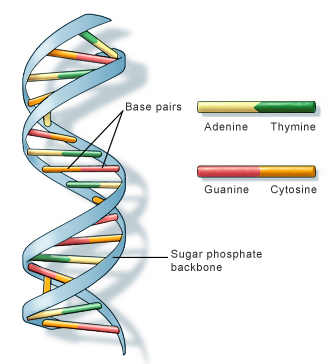
\includegraphics[width=0.45\textwidth]{helix.jpg}
\end{center}

\vspace{5mm}

Each DNA molecule has a special configuration of \emph{nucleotides} that determine what you will look like and how you will act.\cite{pearson}
There are enough miles of DNA wound up in each of us to make it \emph{to the Sun and back} 600 times!
That is a lot of tape to stick data on, and you see the manifestation of that variation in the flora and fauna of planet Earth.
There are a lot of different options available to genetics, and we will look at some of them and how varied they are later in the article.

\subsection{Nucleobases and nucleotides}
\initial{N}ucleotides are worth knowing a little about, given how important they are to you and your uniqueness.
Biology considers four molecules to be the building blocks of everything else: carbohydrates, lipids (fats), proteins and nucleic acid.
We are interested in the acid - this is the defining element of DNA, which in turn is the defining element of us.
In the acid of DNA we find \emph{nucleobases}, which are the smaller jigsaw pieces of the bigger jigsaw puzzle that is DNA.
There are four kinds of nucleobases in DNA - you have most likely seen their abbreviations before; A for adenine, C for cytosine, G for guanine and T for thymine \cite{hankgreen}.
These four nucleobases bind to sugar and a phosphate group in various patterns to form a \emph{nucleotide}.
The order of the nucleotides in the DNA helix is what gives you brown hair, or good muscles for climbing, or an acute sense for pattern recognition, even how wet or dry your earwax is \cite{hankgreen}.
It is all determined by little sequences of acids in the core of your many cells.

The DNA helix is given structure by the sugar.
The sugar is what the nucleotides attach to, which can have some different configurations, and the little nucleotide units connected to sugar are again connected to each other by the phosphate.
In summary, the nucleobases with their many different configurations form the rungs of the DNA ladder \cite{lewontin}.
The sugar and the phosphate are the rails that binds the rungs together.

\subsection{Enzymes}
\initial{I}t is worth mentioning enzymes for how important they are to your body.
Enzymes are, in short, your body's power tools \cite{hankgreen2}.
They are catalysts that speed up chemical reactions.
Pepsin, for example, is the enzyme that lives in your stomach acid and digests your food.
In your mouth you have amalyse, which breaks down starch.
Each little enzyme has an "active site" - where the power tools are put to use - that allows the enzyme to either break a molecule into parts, or reversely, collect smaller molecules into a newer, lager compounds.
These enzymes make our world go round, and since they can put on different hats and work different areas, we have comparatively few of them.
Enzymes are key in cell division, which is how life multiplies. 

\subsection{Cell division and copying}
\initial{I}n short, the way we go from a few cells to many cells to human being, is by splitting the DNA that defines us and subsequently copying that DNA.
This is where the enzymes come in handy, as they can split the DNA strand.
The enzyme responsible for splitting it up is called the helicase.
It moves down the rungs of the ladder and neatly breaks up the DNA strand, and two new and distinct single strands are formed.
Each need to be complemented with the correct nucleobase to complete the same pattern it had before.
Now, without getting too hardcore on the details, the DNA helix is split into two different strands: the leading strand and the lagging strand \cite{hankgreen}.

What seperates the two is how the nucleotides are tied to the sugar molecule - worth looking up if you want more details on the complexity of the DNA molecule \cite{lewontin}.
For now, we will look only at what happens during cell division.

\begin{center}
	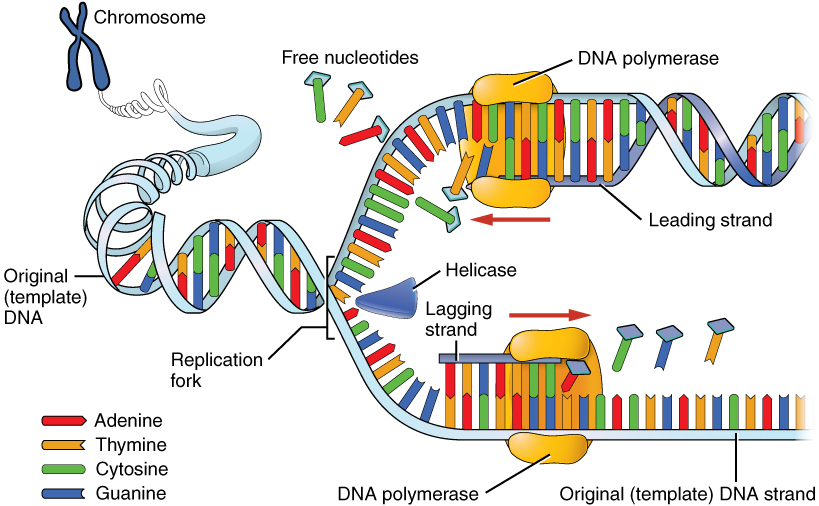
\includegraphics[width=0.45\textwidth]{dna_replication.jpg}
\end{center}

The leading strand has it easiest.
After the helicase enzyme has made its cutting way through, another enzyme called an RNA primer moves on down the line after it.
It has a sniff around about what kind of nucleobases are hanging in the breeze, and makes a few sample connections, leaving a blueprint.
After it is done, the DNA primer hands the rest of the factory work off to another enzyme called DNA polymerase.
The polymerase lumbers on down the entire strand after that, reading the blueprints from the primase, and builds the corresponding nucleobases where they are needed. 

Things are bit more chaotic on the lagging strand.
Here, the order of the nucleobases is not as easily readable.
The RNA primase, the blueprints boss of the DNA split, has to rush back and forth all over the strand to write different blueprints.
The DNA polymerase follows after the primase, huffing and puffing, and builds small subsections of the strand until construction is complete.

The final coat of paint is called DNA ligase, which solidifies the structure of the new-born DNA molecule.
Et voilà, we have the miracle of reproduction at a cellular level \cite{hankgreen}.
This, however, is also where things can go wrong.
Mistakes are made - once every 10th billion nucleotide or so - the construction team messes up and builds a window where a wall should have been, or a tower where a roof should have been.
This is genetic mutation.
Mutation is the reason why we have centipedes and monkeys.